\documentclass[a4paper]{article}

\usepackage[portuguese]{babel}
\usepackage[utf8]{inputenc}
\usepackage{graphicx,hyperref}
\usepackage{float}
\usepackage{listings}
\usepackage{proof,tikz}
\usepackage{algorithm2e}
\usepackage{amssymb,amsthm,stmaryrd}


\usepackage[edges]{forest}
\usetikzlibrary{automata, positioning, arrows}


\newtheorem{Lemma}{Lema}
\newtheorem{Theorem}{Teorema}
\theoremstyle{definition}
\newtheorem{Example}{Exemplo}
\newtheorem{Definition}{Definição}
\newtheorem{Fact}{Fato}


\usepackage{fancyhdr}
  \pagestyle{fancy}
  \fancyhf{}
  \lhead{Teoria da Computação}
  \rhead{Aula 22}
  \lfoot{Prof. Rodrigo Ribeiro}
  \rfoot{\thepage}
  \renewcommand{\footrulewidth}{0.4pt}
  \pagestyle{fancy}

\tikzset{
        ->,  % makes the edges directed
        >=stealth', % makes the arrow heads bold
        node distance=3cm,
        every state/.style={thick, fill=gray!10},
        initial text=$\,$
        }
  

\begin{document}

\title{Aula 22 - A Tese de Church-Turing, codificação de problemas e a MT universal}
  \author{Rodrigo Ribeiro}

  \maketitle

  \pagestyle{fancy}


  \section*{Objetivos}

  \begin{itemize}
     \item Apresentar a tese de Church-Turing.
     \item Discutir como instâncias de problemas podem ser representadas como
           uma linguagens sobre $\Sigma$.
     \item Apresentar a máquina de Turing universal.
  \end{itemize}


  \section{A tese de Church-Turing}

  \begin{Definition}
    Se uma função é computável, então ela é computável por meio de uma máquina
    de Turing.
  \end{Definition}

  A definição anterior expressa que MTs são capazes de expressar \textbf{TODO}
  algoritmo. Em nosso estudo de decidibilidade, estaremos interessados em
  problemas de decisão, visto que esses possuem a mesma dificuldade que suas
  versões convencionais. Porém, para que uma MT solucione um problema decisão, é
  necessário que sua entrada seja expressa usando uma palavra sobre o alfabeto
  da MT em questão. Abordaremos o problema de codificação na próxima seção.


  \section{Codificação de Problemas}

  \begin{Definition}
    Um código para uma instância de um problema de decisão $P$ sobre um alfabeto
    $\Sigma$ consiste de uma palavra $w\in\Sigma^*$ que deve atender
    os
    seguintes requisitos:
    \begin{itemize}
      \item Para cada instância $p$ do problema $P$ deve existir pelo menos uma
        palavra de $\Sigma^*$ que a represente.
      \item Cada palavra de $\Sigma^*$ deve representar no máximo uma instância
        de $P$.
      \item Para cada palavra $w\in\Sigma^*$, deve ser possível determinar se
        $w$ representa ou não uma instância de $P$. 
    \end{itemize}
  \end{Definition}
  
  \begin{Example}
    Considere o seguinte problema de decisão: ``Dado um número $n\in\mathbb{N}$,
    determinar se $n$ é primo''. Apresentaremos duas possíveis representações
    das instâncias deste problema:
    \begin{itemize}
       \item Para cada instância, ``determinar se $n$ é primo'', existe uma
         palavra em $\{1\}^*$ que a representa: $1^n$. A seguir apresentamos que
         requisitos anteriores são atendidos por essa representação.
         \begin{itemize}
           \item Para cada $n \in\mathbb{N}$, existe uma palavra que a
             representa: $1^n$.
           \item Cada palavra $1^n$ representa uma instância do problema
             ``determinar se $n$ é primo''.
           \item Para cada $w \in\{1\}^*$, é possível determinar se ela
             representa ou não uma instância: toda palavra representa uma
             instância do PD.
           \end{itemize}
         \item Usando $\Sigma=\{0,1\}$ podemos representar cada instância usando
           sua representação em binário. Com isso:
           \begin{itemize}
             \item Cada instância é representada por inúmeras palavras, pois
               pode-se adicionar uma quantidade qualquer de 0s à esquerda da
               palavra e não alterar o número que ela representa.
             \item Cada palavra $w \in \{0,1\}^*$ representa, no máximo, uma
               instância. Note que $w = \lambda$ não representa instância
               alguma.
             \item É possível determinar se uma palavra representa ou não uma instância.
           \end{itemize}
    \end{itemize}
  \end{Example}

  Nos próximos exemplos, utilizaremos a notação $R\langle v_1,...,v_n \rangle$
  para representar uma instância de um problema de decisão com $n$ parâmetros.
  Uma MT que resolve o problema em questão receberá $R\langle v_1,...,v_n
  \rangle$ como entrada e para em estado final caso a resposta para o problema de decisão seja
  sim, e em estado não final (ou entra em loop) caso a resposta seja não. A
  figura abaixo ilustra esse fato.

  \begin{figure}[!htb]
    \centering
    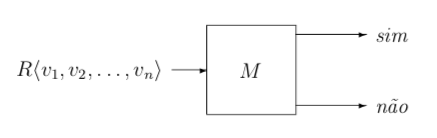
\includegraphics[scale=.6]{MT1.png}
    \caption{MT para problema de decisão.}
  \end{figure}


  A seguir, apresentamos um exemplo mais elaborado de representação de instâncias.

  \begin{Example}
    Considere o problema ``determinar se uma gramática livre de contexto $G$
    gera uma palavra $w$, para $G$ e $w$ arbitrários''. Para apresentarmos a
    codificação deste problema, vamos usar como exemplo a seguinte GLC:

    \[
      \begin{array}{lcl}
        A & \to & aAa \,|\, B \\
        B & \to & aB \,|\, CC \\
        C & \to & b \,|\,\lambda 
      \end{array}
    \]

    Uma possível codificação é como se segue. Considere $G = (V,\Sigma_G,R,P)$
    em que $V = \{A_1,...,A_n\}$ e $\Sigma_G =\{a_1,...,a_m\}$. Representaremos
    a entrada para o problema de decisão acima mencionado como uma palavra
    sobre $\{0,1\}$. Para isso, precisamos encontrar uma maneira de representar
    cada um dos componentes de uma gramática $G$. Faremos isso da seguinte maneira:
    \begin{itemize}
       \item Representaremos uma variável $A_i$, $1 \leq i \leq n$, por $1^i$.
         Na gramática anterior, temos que representaremos a variável $A$ por 1,
         $B$ por 11 e $C$ por 111.
       \item Representaremos um símbolo do alfabeto $a_j$, $1 \leq j \leq m$,
         por $1^{n + j}$. Dessa forma, temos que o símbolo $a$ será representado
         por $1^{3+1} = 1^4$ e $b$ por $1^{3 + 2} = 1^5$.
       \item Representaremos regras como uma sequência dos códigos dos simbolos
         que a compõe separados por 0. Como exemplo, considere a regra $A \to
         aAa$. Essa seria representada por
         $R\langle A \rangle 0 R\langle a \rangle 0 R\langle A \rangle 0
         R\langle a \rangle = 1 0 1^4 0 1 0 1^4$.
       \item Representamos o conjunto de regras de uma gramática separando o
         código correspondente a cada regra usando a palavra 00. Como exemplo,
         anteriormente apresentamos o código para a regra $A \to aAa$, que é:
         \[
           R\langle A \rangle 0 R\langle a \rangle 0 R\langle A \rangle 0
            R\langle a \rangle
         \]
         Por sua vez, a regra $A \to B$ é representada como:
         \[
           R\langle A \rangle 0 R\langle B \rangle
         \]
         A sequência dessas duas regras é representada como:
         \[
           R\langle A \to aAa \rangle 00 R\langle A \to B \rangle
         \]
       \item Finalmente, a representação completa da gramática é dada por:
         $R\langle (V,\Sigma_G,R,P)\rangle = 1^n01^m0 R\langle R \rangle$, em
         que $R\langle R \rangle$ é a representação do conjunto de regras de
         $G$, $n$ é o número de variáveis e $m$ o número de símbolos do alfabeto.
     \end{itemize}
     Com base na representação acima, podemos definir a instância do problema de
     decisão deste exemplo como $R\langle G, w \rangle = R\langle G \rangle 000
     R\langle  w \rangle$, em que $R\langle G \rangle$ é a codificação da
     gramática e $R\langle w \rangle$ é a representação da palavra de entrada.  
  \end{Example}

  \section{Máquina de Turing Universal}

  Nessa seção discutiremos uma possível codificação de MTs que permita a
  construção de uma MT capaz de simular MTs recebidas como um código em sua fita
  de entrada. A MT capaz de executar outras MTs é denominada MT Universal. A
  definição seguinte apresenta essa possível codificação, seguida de um exemplo.

  \begin{Definition}[Codificação de MTs]
    Seja $M = (E,\Sigma,\Gamma,\langle, \sqcup, \delta,i,F)$ uma MT qualquer, em
    que $E = \{e_1,...,e_n\}$, $\Gamma = \{a_1,...,a_m\}$, $i = e_1$, $a_1 =
    \langle$, $a_2 = \sqcup$ e $F = \{f_1,...,f_p\}$. Representaremos cada
    estado $e_i$ por $R\langle e_i \rangle = 1^i$. De maneira similar,
    representaremos símbolos de $\Gamma$: $R\langle a_i \rangle = 1^i$.
    Representaremos a direção para mover o cabeçote da seguinte maneira:
    $R\langle E \rangle = 1$ e $R\langle D \rangle = 11$. Dado o exposto,
    a representação de $M$ (supondo que $M$ possui transições $t_1, ...,t_s$) é:
    \[
      R\langle M \rangle = R\langle F \rangle 00 R\langle
      t_1 \rangle 00 ... 00 R\langle  t_s \rangle
    \]
    em que $R\langle F \rangle$ é a representação dos estados finais de $M$, que
    pode ser feita seperando o código de cada estado usando o símbolo 0:
    \[
      R\langle F \rangle = R\langle f_1 \rangle 0 ... 0 R\langle f_p \rangle
    \]
    Cada transição $t$ da forma $\delta(e,a)=[e',b,d]$ é representada como:
    \[
      R\langle e \rangle 0 R\langle a \rangle 0 R\langle e' \rangle 0 R\langle b
      \rangle R\langle d \rangle
    \]
  \end{Definition}

  Apresentamos um exemplo da codificação apresentada.

  \begin{Example}
    Considere a seguinte MT $M = (\{A,B\},\{a,b\},\{\langle, \sqcup,
    a,b\},\langle, \sqcup, \delta, A, \{A,B\})$.
    \begin{figure}[H]
      \begin{tikzpicture}
        \node[state, initial, accepting](s0){$A$} ;
        \node[state, accepting, right of=s0](s1){$B$};
        \draw (s0) edge[above, bend left]node{$a/a\:D$}(s1)
              (s1) edge[below, bend left]node{$b /b\: E$} (s0);
      \end{tikzpicture}
      \centering
    \end{figure}
    Usando a codificação anterior, temos a seguinte representação dos estados e
    símbolos do alfabeto:
    \begin{itemize}
      \item $R\langle A \rangle = 1$, $R\langle B \rangle = 11$.
      \item $R\langle a \rangle = 1^3$, $R\langle b \rangle = 1^4$.
    \end{itemize}
    A transição $t_1$, $\delta(A,a) = [B,a,D]$, é representada por:
    \[
      R\langle A \rangle 0 R\langle a \rangle 0 R\langle B \rangle 0 R\langle a
      \rangle 0 R\langle D \rangle
    \]
    Por sua vez, a transição $t_2$, $\delta(B,b) = [A,b,E]$, é representada como:
    \[
      R\langle B \rangle 0 R\langle b \rangle 0 R\langle A \rangle 0 R\langle b
      \rangle 0 R\langle E \rangle
    \]
    Seguindo a codificação apresentada, temos que a MT acima possui a
    codificação:
    \[
      R\langle A \rangle 0 R\langle B \rangle 00 R\langle t_1 \rangle 00 R\langle t_2 \rangle
    \]
  \end{Example}

  Após apresentarmos a codificação de MTs, podemos descrever uma MT que é capaz
  de simular outras MTs fornecidas como entrada em sua fita.

  \begin{Definition}[Máquina de Turing Universal]
    A MT universal é uma MT de 3 fitas que:
    \begin{itemize}
      \item A fita 1 possui a palavra de entrada $R\langle M,w \rangle$, que
        representa a máquina $M$ a ser simulada e a palavra $w$ a ser processada
        por $M$.
      \item A fita 2 é usada para simular a computação de $M$ sobre a fita
        contendo $w$. Isto é, a fita 2 representa a fita de $M$.
      \item A fita 3 armazena o estado atual de $M$.
      \end{itemize}
      A MT universal é descrita pelo seguinte algoritmo:

      
      \begin{algorithm}[H]
        Copie $R\langle w \rangle$ na fita 2 e posicione o cabeçote no início \;
        Escreva $R\langle i \rangle$ na fita 3 e posicione o cabeçote no início\;
        \While{true}{
          Seja $R\langle a \rangle$ a representação sobre o cabeçote na fita 2\;
          Seja $R\langle e \rangle$ a representação sobre o cabeçote na fita 1\;
          Procure $R\langle e \rangle0 R\langle a \rangle 0 R\langle e' \rangle
          0 R\langle b \rangle 0 R\langle d \rangle$ na fita 1 \;
          \eIf{encontrou}{
            Substitua $R\langle e \rangle$ por $R\langle  e' \rangle$ na fita 3
            e volte seu cabeçote ao início \;
            Substitua $R\langle a \rangle$ por $R\langle b \rangle$ na fita 2 \;
            Mova o cabeçote da fita 2 na direção $d$ \;
          }{
            Pare \;
          }
        }
      \end{algorithm}
  \end{Definition}

  Denominados a MT universal por $U$. Observe que a linguagem aceita por $U$ é:

  \[
    L(U) = {R\langle M,w \rangle \,|\, M \textit{para com entrada }w}.
  \]

  Veremos na próxima aula que essa linguagem é um exemplo de linguagem
  recursivamente enumerável (existe uma MT que a aceita, $U$) que não é
  recursiva, pois existem entradas que fazem $U$ não terminar sua computação.
  
  \section{Exercícios}

  \begin{enumerate}
     \item Apresente uma codificação para os seguintes problemas de decisão:
       \begin{enumerate}
         \item Dado um AFD $M$ e uma palavra $w$, determinar se $w \in L(M)$.
         \item Dado um grafo $G$, determinar se $G$ pode ser colorido usando $k$
           cores.
       \end{enumerate}
      \item Mostre que a linguagem $\{R\langle M,w \rangle\,|\,M\textit{ passa
          duas vezes por algum estado de }M\}$ é recursiva.  
  \end{enumerate}
\end{document}
